Neste capítulo é apresentado o sistema Decisioner, principal contribuição
do projeto desenvolvido, ele gerá Sistemas de Apoio à Decisão e está
composto por ontologias para representar o conhecimento e por uma
DSL que permite gerenciar os conceitos e estabelecer as configurações
gerais por parte de especialistas do domínio para gerar o SAD.

Os SADs segundo a descrição feita no capitulo \ref{chap:Context}
estão compostos por banco de dados, base de modelos, base de conhecimento
e a GUI como componentes principais, os quais foram organizados em
componentes baseados na Web Semântica e nas DSL com a finalidade de
desenhar um sistema gerador de SAD. 

\section{Arquitetura do Decisioner}

A arquitetura de um software define a organização em termos de seus
componentes, suas interconexões, suas interações e também suas principais
propriedades \citet{de1997software}. Ela fornece as informações de
como os elementos envolvidos nela se relacionam. Arquiteturas trabalham
a parte externa das ligações entre seus elementos, implementações
internas desses elementos não são considerados arquiteturais \citet{sei2006architecture}.

Para encontrar e configurar componentes de software de uma arquitetura,
uma opção é descrever esses componentes, usando uma ontologia, e usar
os termos dessa ontologia para encontrar os componentes corretos para
uma aplicação \citet{Linhalis2010}. Essas ontologias podem ser criadas
utilizando linguagens padrões da Web Semântica, como a Web Ontology
Language (OWL), para melhor portabilidade \citet{Pahl2007}. Ontologias
e padrões da Web Semântica serão abordados com mais profundidade no
próximo capítulo.

Devido ao fato de que os elementos básicos de todo o SAD (Figura \ref{fig:Componentes-SAD})
serem muito parecidos, é possível criar uma arquitetura que possa
ser re\nobreakdash-usada em diferentes SADs (ou classes de SADs).
Esta arquitetura pode ser baseada em componentes de software re\nobreakdash-usáveis.
Programadores podem usar essa arquitetura e re\nobreakdash-usar os
componentes de software, já desenvolvidos para ela, para implementar
SADs mais rapidamente.

Como especialistas de domínio não têm um conhecimento muito detalhado
sobre linguagens de especificação de sistemas, é necessário o desenvolvimento
de uma \foreignlanguage{english}{Domain Specific Languag}e (DSL) adequada
ao nível de conhecimento de computação dos especialistas. Essa linguagem
também deve conter termos familiares ao domínio desses especialistas. 

Após uma pesquisa bibliográfica não foi possível encontrar sistemas
que propusessem a geração automática de interface para Sistemas de
Apoio a Decisão (SADs) com ou sem o uso de ontologias. Os artigos
encontrados mais próximos ao tema deste trabalho tratam do uso de
ontologias ou de frameworks em SADs para a área de sustentabilidade,
área que vai ser usada neste trabalho para teste dos sistemas desenvolvidos. 

O modelo geral desta solução é apresentado na Figura \ref{fig:Interfaces},
na qual as ontologias representam o banco de dados, base de modelos
e base de conhecimento, permitindo a integração e padronização desses
componentes, ditas ontologias são gerenciadas pela DSL que permite
definir o comportamento do SAD e finalmente é integrado o sistema
de GUIs que permite visualizar o SAD por meio de uma interface Web,
suportando assim o componente visual dos SAD.

O processo de definição dos SAD são controlados pela DSL, disponibilizando
aos especialistas do domínio uma linguagem especializada e de fácil
uso para definir e configurar os SAD segundo o critério deles, o conjunto
destes três componentes foi intitulado Decisioner.

\begin{figure}[H]
\centering{}\includegraphics[width=0.8\columnwidth]{\string"figures/Decisioner Architecture\string".png}\caption{Arquitetura do Decisioner\label{fig:Interfaces}}
\end{figure}

\begin{enumerate}
\item Ontologia de interfaces gráficas: ontologia que representa as interfaces
gráficas de usuários e os tipos de dados, fazendo um mapeamento entre
os dois.
\item TripleStore: sistema de armazenamento e recuperação da informação
que padroniza as informações em formato de triplas, permitindo a compatibilidade
e o reúso das informações entre fontes de dados externas.
\item Sistema gerador de interfaces gráficas: Sistema que usa a ontologia
de interfaces gráficas e as definições feitas na DSL para gerar as
interfaces gráficas Web, que compõem os SADs gerados pelo Decisioner.
\end{enumerate}

\section{Trabalhos relacionados}

Sobre as ontologias na interface gráfica encontramos: no artigo de
\citet{ruiz2006using} é analisado o uso de ontologias na engenharia
de software, identificando 50 tipos de uso entre as quais foram identificados
dois usos no suporte de interfaces gráficas.

\citet{paulheim2012ontology} propõem a seguinte definição, uma \foreignlanguage{english}{ontology-enhanced
user} interface é uma interface cujas capacidades de visualização,
possibilidades de interação, ou processo de desenvolvimento estão
habilitados ou (pelo menos) melhorado pelo emprego de uma ou mais
ontologias, na pesquisa foram identificados três propósitos para os
quais são usadas as ontologias no melhoramento das interfaces gráficas,
e são os seguintes:
\begin{enumerate}
\item Melhorar as capacidades de visualização;
\item Melhorar as possibilidades de interação;
\item Melhorar o processo de desenvolvimento;
\end{enumerate}
são apresentados os usos mais comuns de ontologias que suportem interfaces
gráficas (ontology-enhanced user interface), eles

\section{Metodologia}

Com a finalidade de desenvolver o modelo de geração de SAD anteriormente
dito, foi escolhido um caso de uso que corresponde a um SAD para avaliação
da sustentabilidade intitulado SustenAgro, o qual foi requerido pelos
especialistas em sustentabilidade da Embrapa Meio Ambiente.

O desenvolvimento dos componentes do Decisioner foram realizados da
seguinte maneira:
\begin{enumerate}
\item Seleção da \foreignlanguage{english}{Triplestore}: foi realizado um
processo de avaliação das \foreignlanguage{english}{triplestores}
existentes com a finalidade de definir uma que adapta-se nos requisitos
do sistema Decisioner.
\item Seleção da linguagem de programação e framework web: foi realizado
uma verificação das tecnologias de desenvolvimento de sistema web
compatíveis com as tecnologias da web semântica e com as DSLs.
\item Design da DSL:
\item Desenvolvimento do interprete DSL:
\item Integração com tencologias de Web Components:
\item Desenvolvimento de modulo de geração de GUIs.
\item Desenvolvimento do DSL editor:
\item Desenvolvimento do Ontology Editor:
\end{enumerate}
Os componentes da arquitetura do SustenAgro não são exclusivos do
SustenAgro, podendo ser reusados em outros SADs, os quais foram generalizados
para suportar a geração de outros tipos de sistema.

\subsection{Ontologia Decisioner}

Sobre as ontologias sobre interfaces gráficas, no artigo de \citet{ruiz2006using}
é analisado o uso de ontologias na engenharia de software, identificando
50 tipos de uso entre os quais foram identificados dois usos no suporte
de interfaces gráficas.

\citet{paulheim2012ontology} propõem a seguinte definição, uma \emph{ontology-enhanced
user interface} é uma interface cujas capacidades de visualização,
possibilidades de interação, ou processo de desenvolvimento estão
habilitados ou, pelo menos, melhorados pelo emprego de uma ou mais
ontologias. Na pesquisa foram identificados três propósitos para os
quais são usadas as ontologias no melhoramento das interfaces gráficas:
\begin{enumerate}
\item Melhorar as capacidades de visualização;
\item Melhorar as possibilidades de interação;
\item Melhorar o processo de desenvolvimento;
\end{enumerate}
Foram apresentados também os usos mais comuns de ontologias que suportam
interfaces gráficas (ontology-enhanced user interface).

Além disso, na literatura, existem pesquisas relacionadas com o vocabulário
\emph{AGROVOC Agricultural Vocabulary} \footnote{http://aims.fao.org/agrovoc}
que é um \foreignlanguage{english}{\emph{thesaurus}} que fornece termos
padronizados sobre alimentação, nutrição, agricultura, pesca, floresta
e meio ambiente criados de maneira colaborativa e coordenados pela\emph{
}\foreignlanguage{english}{Food and Agriculture Organization} (FAO\nomenclature{FAO}{Food and Agriculture Organization}).
Esses termos podem ser reutilizados nas ontologias \citep{DCMIPro841},
permitindo uma padronização dos identificadores dos conceitos, reutilizando
informações e integrando os conceitos com outros dados. Essa reutilização
foi feita através da vinculação da AGROVOC ao sistema \emph{AOS/CS
Agricultural Ontology Service Concept Server}, a FAO desenvolveu um
modelo base para esse novo sistema utilizando o \emph{OWL Web Ontology
Language.}

Cada uma destas pesquisas fornece um exemplo do uso das tecnologias
da web semântica na criação de soluções baseadas em conhecimento.
Isso é confirmado por \citet{roussey2010ontologies} por meio da descrição
de (i) como as ontologias têm sido usadas para múltiplas tarefas,
uma das quais é conseguir interoperabilidade entre sistemas de informação
heterogêneos; e de (ii) como as seguintes gerações de sistemas de
informação utilizariam uma base do conhecimento do domínio. Dadas
as afirmações dessas pesquisas, pode-se deduzir que uma ontologia
pode proporcionar o suporte conceitual para cumprir os requisitos
de sistema SAD, como o SustenAgro.

A ontologia de Sistema Apoio à Decisão contem os elementos que foram
abstraidos a partir do analise dos sistemas SAD usados pela Embrapa
Meio Ambiente em seus processos de avaliação.

Os sistemas software de avaliação que foram analisados foram:
\begin{enumerate}
\item Sistema SustenAgro: avaliação da sustentabilidade agricola em cana-de-açúcar.
\item Sistema Innova-Tec: avaliação do impacto da inovação tecnológica.
\item Sistema Nano-Tec: avaliação do impacto das nanotecnologias.
\end{enumerate}
A partir desses sistemas foram identificados elementos comuns, que
foram abstraidos na ontologia SAD com o proposito de generalizar as
classes da ontologia sustenagro, para fornecer a geração de interfaces
gráficas .

As classes idenficadas e modeladas são:
\begin{itemize}
\item Evaluation Object: classe que representa os objetos que serão analisados
em cada processo de avaliação, os quais vão ficar como indivíduos
desta classe ou de alguma subclasse dela, no caso do sistema SustenAgro
a classe \textit{Production Unit }é subclasse do Evaluation Object.
\item Feature: classe que representa as caraterísticas de um Evaluation
Object que serão quantificadas, analisadas e usadas no processo de
geração de resultados do processo de avaliação, pelo geral as Features
tem uma propriedade numérica que a quantifica.
\item Analysis: classe que vincula o resultado de uma avaliação, o nome
e data da avaliação, assim como o Evaluation Object, para representar
uma avalição
\item Value: classe que representa os valores que são atribuídos a cada
instancia de Feature.
\item User: classe que representa os usuários do sistema.
\item Role: classe que representa os tipos de usuário do sistema, relacionando
as permissões de cada tipo, por padrao tem estão instanciados os perfis
User e Admin
\end{itemize}
Na figura \ref{fig:Modelagem-do-SAD} é apresentada a modelagem basica
da estrutura de um SAD, com as classes que foram obtidas a partir
da abstração da ontologia SustenAgro.

\begin{figure}[H]
\centering{}\includegraphics[scale=0.5]{\string"figures/DSS ontology\string".png}\caption{Modelagem abstracto do SAD\label{fig:Modelagem-do-SAD}}
\end{figure}

A classe \textit{Value }representa os valores que são relacionados
com cada característica da unidade produtiva, o qual esta subdividido
nas classes \textit{Categorical }ou \textit{Real, }no caso de SustenAgro
representa os possíveis valores que um \textit{Indicator} ou \textit{Variable}
pode ter, os elementos discretos e definidos como os categóricos são
modelados como indivíduos da classe, permitindo assim, restringir
as opções de escolha.

Na figura \ref{fig:Modelagem-de-Value} é apresentado a classe \textit{Value}
e as subclasses modeladas, tanto \textit{Categorical} para conjunto
finito de valores e \textit{Real} para valores numéricos, como exemplo
está a classe \textit{Yes/No} que representa os valores de sim e não,
os quais são modelados como indivíduos de dita classe.

Cada individuo da classe \textit{Value} tem a propriedade \textit{as
number }que relaciona um valor numérico para definir um critério de
comparação e fornecer um formato para este tipo de dados.

\begin{figure}[H]
\begin{centering}
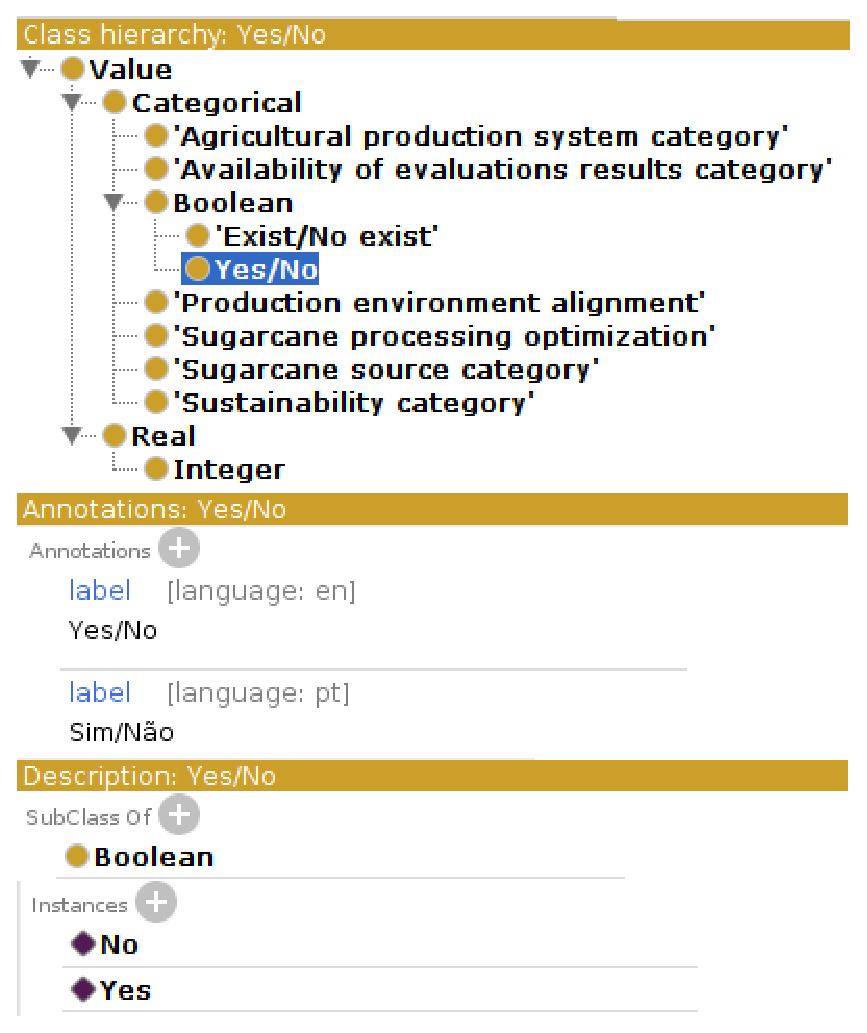
\includegraphics[scale=0.5]{figures/Value}
\par\end{centering}
\caption{Modelagem de Value\label{fig:Modelagem-de-Value}}
\end{figure}

Estas classes são complementadas com propiedades como rdfs:range ou
por padrões dos dados que relacionam as widgets mais apropriadas na
representação de informações, e assim fornecer a geração de interfaces
graficas de usuário.

A partir do anterior formato a classe 

Para definir a ontologia de domínio do SustenAgro, realizou-se uma
pesquisa das fontes de dados relacionadas com ontologias do domínio
de avaliação de sustentabilidade em sistemas produtivos de cana-de-açúcar.
Concluiu-se que não existem ontologias que suportem esse domínio,
por isso propõe-se desenvolver uma ontologia que utilize os conceitos
de avaliação de sustentabilidade e de sistemas agrícolas. Ela deve
fazer uso da pesquisa realizada por \citet{oliveira:2013} e de algumas
tecnologias fornecidas pela FAO. Essa ontologia terá a finalidade
de fornecer uma base conceitual e tecnológica para suportar o processo
de avaliação de sustentabilidade no sistema produtivo da cana\nobreakdash-de\nobreakdash-açúcar
no estado de São Paulo.

O desenvolvimento dessa ontologia ocorrerá de forma ágil e modular,
por meio de técnicas de prototipação rápida, que serão de âmbito e
complexidade crescente, abrangendo grupos de conceitos relacionados
entre si.

O desenvolvimento da ontologia depende essencialmente da comunicação
entre os especialistas e os modeladores. Foram definidos meios de
comunicação e de representação do conhecimento: reuniões presenciais
e virtuais, e o modelos conceituais que permitem uma visualização
direta do domínio.

Inicialmente, o modelo conceitual vai ser representado por meio de
um mapa conceitual que permitirá a comunicação em um formato reconhecido
por cada um dos profissionais envolvidos no projeto. Esse modelo será
representado em OWL (pelos modeladores) e serão definidas instâncias
para cada uma das classes. Depois disso, o especialista do domínio
construirá perguntas de interesse, com as quais os modeladores definirão
consultas que o sistema deverá responder segundo os resultados esperados,
conseguindo validar e ajustar até ter um protótipo confiável.

O conhecimento do domínio envolvido no sistema Sustenagro está em
contínua construção. Por isso, é necessário um enfoque que permita
realizar mudanças na estrutura e no conteúdo usados no sistema durante
seu desenvolvimento. As ontologias permitem representar o conhecimento
de um domínio por meio de formatos, como a linguagem OWL, permitindo
separar o conhecimento das outras partes do sistema.

A ontologia do domínio foi desenvolvida baseada nas definições feitas
pelos especialistas, que foram generalizadas a través das seguintes
classes representadas na Figura \ref{fig:StructureOfDomainOntology},
cada uma delas permite representar os conceitos gerais dos sistemas
de avaliação da sustentabilidade.

Também permite a integração de conceitos, inclusive quando pertencem
a domínios sem relação aparente. Um exemplo disso é a inter-relação
do conhecimento de sustentabilidade com conhecimento de interfaces
gráficas de usuário, que suporta a geração de SAD para avaliação da
sustentabilidade, o conhecimento modelado foi dividido em duas ontologias,
avaliação de sustentabilidade e do SAD.

As ontologias da web semantica são compatíveis com as tecnologias
web, permitindo o uso e integração por outros sistemas dado que está
em um formato padronizado.

\begin{figure}
\begin{centering}
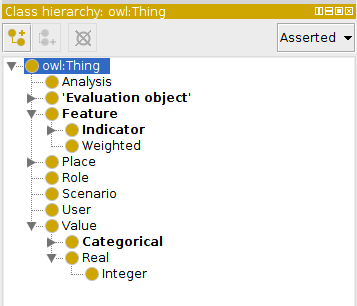
\includegraphics[scale=1.5]{figures/StructureOfDomainOntology}
\par\end{centering}
\caption{Estrutura Geral da Ontologia de Domínio\label{fig:StructureOfDomainOntology}}
\end{figure}

A classe \foreignlanguage{english}{\textit{Analysis}} representa o
conceito de avaliação de sustentabilidade onde cada individuo dela
representa uma avaliação cadastrada no sistema. 

A classe \foreignlanguage{english}{\textit{EvaluationObject}}\textit{
}representa os objetos que serão avaliados pelo SAD, os quais tem
indicadores que permitem suportar o processo de avaliação.

A classe \foreignlanguage{english}{\textit{Feature}} representa cada
uma das características dos objetos de avaliação, principalmente indicadores
que são usados durante o processo de avaliação

A classe \foreignlanguage{english}{\textit{Indicator}} representa
o conceito de indicador que representa cada conceito a avaliar

A classe \foreignlanguage{english}{\textit{Weighted}} representa o
conceito de indicador vinculado com um peso que permite atribuir uma 

Ontologia de controles de gráficos: a finalidade dessa ontologia é
dar suporte a composição de controles gráficos relacionados com os
indicadores. Esse é um requisito funcional do software, uma vez que
os indicadores podem ter diversos tipos de unidades e para cada tipo
existe um tipo de controle gráfico mais apropriado para sua representação.
Por exemplo, para representar um indicador de sustentabilidade do
tipo numérico é recomendável usar um controle visual tipo spinner.

O sistema gerador de interfaces gráficas permite suportar aspectos
de usabilidade e flexibilidade ao sistema. Essa última característica
constitui uma nova proposta de desenvolvimento de SADs que permite
a adaptação automática (ou semi\nobreakdash-automática) da interface
às mudanças dos conceitos do domínio.

Será desenvolvida uma ontologia para interfaces gráficas focada na
definição e modificação de controles de usuário. Um exemplo do uso
dessa ontologia é nos indicadores. Eles armazenam um valor inserido
pelo usuário, que pode ser de diversos tipos como numérico continuo,
numérico discreto, percentagem, booleano, lista de termos ou alfanumérico.
Dada essa diversidade, é importante representar os diversos tipos
de controles gráficos em uma linguagem do domínio do especialista,
para que possam ser usados para \foreignlanguage{english}{input} da
definição dos indicadores e que faça um mapeamento entre os indicadores
e os tipos de indicador que vai ser armazenado no sistema.

Esta ontologia vai suportar a DSL fornecendo uma definição formal
dos controles gráficos que serão mapeados para cada tipo de indicador,
a DSL será apresentada a continuação.

As ontologias desenvolvidas foram modelados os conceitos envolvidos
no processo de avaliação da sustentabilidade em agricultura, definindo,
classificando e relacionando cada um dos conceitos para assim permitir
o uso em outros sistemas e conseguir fazer inferência de novo conhecimento.

\section{Decisioner DSL}

No desenvolvimento da presente pesquisa foi necessário definir uma
DSL que permitisse representar as principais características do SAD
que precisávamos desenvolver, dito SAD foi desenhado para avaliar
a sustentabilidade em agricultura, pelo qual foram integrados conceitos
do domínio de conhecimento na definição dos componentes do SAD, fornecendo
uma linguagem para especialistas onde é suportada a de definição dos
SAD, as características da DSL são:

A DSL foi baseada na linguagem Groovy \citet{koenig2007groovy}, sendo
uma extensão da linguagem Groovy, devido a que esta linguagem suporta
o desenvolvimento de DSLs. Isso inclui suporte a DSL Descriptors,
arquivos Groovy que descrevem extensões \emph{domain-specific} para
o motor de inferência e assistente de conteúdo do plugin Groovy\nobreakdash-Eclipse. 

Uma outra vantagem de Groovy é a disponibilidade do Grails Framework
para a criação de aplicações Web \citet{judd2008beginning}. 

O uso da DSL por especialistas em sustentabilidade deve diminuir o
esforço necessário para se desenvolver um SAD nesse domínio.

Espera-se que, usando a DSL, os próprios especialistas vão ser capazes
de fazer parte do desenvolvimento e validação.

A DSL e o interprete conformam uma ferramenta intitulada Decisioner,
que por meio de umas declarações permite a geração de \nomenclature{SAD}{Sistema de apoio à decisão},
dita ferramenta foi a principal contribuição desta pesquisa.

\subsection{Evaluation Object}

Os SAD focados na avaliação, é necessário definir um objeto de avaliação
que permita representar as entidades a avaliar, este objeto pelo geral
tem propriedades que vão representar cada uns dos indivíduos a avaliar,
pelo qual foi definido o comando \textit{evaluationObject, }que define
a estrutura do objeto de avalização e vincula os controles visuais,
o comando tem como argumentos a URI da classe dos elementos que vão
ser avaliados e cada uma das propriedades relacionadas. No código
\ref{lis:DSL-para-defini=0000E7=0000E3o} apresenta-se uma parte da
DSL que define a classe do objeto de avaliação \textit{ProductionUnit}
e as propriedades por meio dos comandos \foreignlanguage{english}{\textit{instance}}\textit{
}e\textit{ }\foreignlanguage{english}{\textit{type}}\textit{.}

\inputencoding{latin9}\begin{lstlisting}[caption={Defini��o de Evaluation Object  },label={lis:DSL-para-defini=0000E7=0000E3o}]
evaluationObject ":ProductionUnit", {     
 instance "ui:hasName', label: ["en": "Name", "pt": "Nome"]
 instance ":hasAgriculturalProductionSystem"
 type label: ["en": "Type", "pt": "Tipo"]
}
\end{lstlisting}
\inputencoding{utf8}
O comando \foreignlanguage{english}{instance} vincula uma propriedade
definida na ontologia através da URI a qual pode estar complementada
por parâmetros que customizam a representação visual da propriedade.

O comando type vincula as subclasses da classe principal, para ser
atribuida nas intancias de Evaluation Object, no caso do Sistema SustenAgro,
dito comando identifica que as instancias de\textit{ ProductonUnit}
também podem ser um \textit{Provider} ou uma \textit{Plant}. Os parâmetros
que podem complementar os anteriores comandos são:
\begin{enumerate}
\item \textit{label}: define um texto associado
\item \textit{placeholder:} define um texto de ajuda
\item \textit{required}: define uma propriedade obrigatória
\item \textit{widget}: define um controle gráfico de usuário
\end{enumerate}

\subsection{Feature: }

O comando \textit{Feature} define as características que serão apresentadas
durante a avaliação para serem instanciadas como parte da Analysis,
ele tem como argumento uma URI que permite vincular as subclasses
da classe referenciada, as instancias destas classes serão quantificadas
mediante o processo da avaliação no qual é realizado o preenchimento
da propriedade \textit{has value }que vincula cada Feature com um
Value para quantificá-lo. No sistema SustenAgro foram estabelecidas
as Features por meio das URIs das classes: EnvironmentalIndicator,
EconomicIndicator, SocialIndicator, ProductionEfficiencyFeature e
TechnologicalEfficiencyFeature. Além disso é possível acrescentar
a inserção de \foreignlanguage{english}{\textit{features}} novas na
interface gráfica de usuário a través do parâmetro \foreignlanguage{english}{\textit{extraFeatures}}.\inputencoding{latin9}
\begin{lstlisting}[caption={Defini��o de Features}]
feature ':EnvironmentalIndicator', 'extraFeatures': true
\end{lstlisting}
\inputencoding{utf8}

\subsection{Logica de avaliação: }

O comando \textit{Report} define o tratamento quantitativo que vai
ser efetuado às \foreignlanguage{english}{\textit{Features}}, com
a finalidade de obter valores gerais ou padrões como resultado do
processo de avaliação, suportando a definição de operações logicas
e aritméticas existentes tanto das linguagens Java e Groovy, fornecendo
assim uma linguagem para edição do metodo de avaliação, permitindo
atualizar o metodo dinámicamente e em tempo de execução, ditos valores
gerais são apresentados diretamente ou por meio de \foreignlanguage{english}{\textit{widgets}}
que facilitem a representação e compreensão da avaliação do sistema.
No código seguinte apresenta-se a implementação da formula do Sistema
SustenAgro, criando variáveis resultado de operações aritméticas para
gerar resultados gerais, no caso do SustenAgro o código gera a variável
\foreignlanguage{english}{\textit{sustainability}} que representa
o índice de sustentabilidade, más pode ser definido qualquer método
computável.\inputencoding{latin9}
\begin{lstlisting}[caption={Defini��o da logica de avalia��o.}]
report {     
 environment = weightedSum(data.':EnvironmentalIndicator')
 economic = weightedSum(data.':EconomicIndicator')
 social = weightedSum(data.':SocialIndicator')
 sustainability = (environment + social + economic)/3
}
\end{lstlisting}
\inputencoding{utf8}
O comando \foreignlanguage{english}{\textit{report}} também define
as \foreignlanguage{english}{\textit{widgets}} que conformam a parte
visual do \foreignlanguage{english}{\textit{report}}, o qual pode
usar as variáveis de resultado da logica de avaliação como entrada
das \foreignlanguage{english}{\textit{widgets}} para melhorar a representação
e facilitar a compreensão dos resultados. No código seguinte apresenta-se
um exemplo de uso desta funcionalidade no sistema SustenAgro, no qual
são definidos comandos que geram as interfaces gráficas, como \textit{sustainabilityMatrix}
que usa as variáveis geradas anteriormente como argumentos.\inputencoding{latin9}
\begin{lstlisting}[caption={Defini��o dos controles visuais do report}]
report {
 evaluationObjectInfo()
 sustainabilityMatrix x: sustainability, y: efficiency
 text 'en': 'Microregion map', 'pt': 'Mapa da microregi�o'
 map data.'Microregion'
}
\end{lstlisting}
\inputencoding{utf8} Por meio dessas configurações da DSL definiu-se as interfaces gráficas
de usuário do sistema para suportar o processo de avaliação, gerando
a representação visual dos Evaluation Objects, das Features, da logica
da avaliação e da interface gráfica do report.

Esta DSL permitirá que a interface gráfica seja definida em uma linguagem
de alto nível. Ela está baseada nas duas ontologias base e permite
definir e administrar os seguintes elementos conceituais:
\begin{itemize}
\item Indicadores
\item Componentes dos indicadores
\item Limiares
\item Métodos
\item Avaliações
\item Índices
\end{itemize}
Os elementos que compõem a DSL tem controles gráficos predefinidos
e será possível parametrizar as características destes controles gráficos
visuais. Por exemplo para as propriedades de tipo numérico contínuo
tem uma \foreignlanguage{english}{\textit{widget}} que representa
os valores reais que posem ser atribuídos em aquela propriedade, dita
\foreignlanguage{english}{\textit{widget}} pode ser mudada a outra
de acordo com as preferencias dos usuários. No caso das mudanças no
design são feitas através da edição do CSS3.

\section{TripleStore}

O sistema SustenAgro será baseado nas tecnologias da web semântica,
entre as tecnologias existentes encontra-se a Triplestore que é um
banco de dados para o armazenamento e recuperação de triplas \citet{rusher2003triple}.
Para o presente projeto foi selecionada a Triplestore Parliament \footnote{http://parliament.semwebcentral.org/}
porque fornece as características: suporte nativo a SPARQL\nomenclature{SPARQL}{SPARQL Protocol and RDF Query Language}
e SPARQL/Update e implementa o SPARQL Protocol Endpoint. Esse último,
padroniza o armazenamento e recuperação da informação; e a compatibilidade
com os sistemas web por meio do Endpoint.

\section{Sistemas de apóio à decisão}

Os sistemas de apóio à decisão (SAD) ajudam no entendimento de processos
complexos, auxiliam na comparação dos fenômenos envolvidos e suportam
a análise e escolha de alternativas no processo de decisão \citep{heinzle2010semantica}.

A equipe de TI do SustenAgro determinou que o tipo de sistema mais
conveniente para o desenvolvimento seria um Sistema de Apóio à Decisão
(SAD). Com a finalidade de definir a arquitetura e a interface gráfica
desse sistema realizaram-se duas perguntas de pesquisa que orientaram
esse projeto:
\begin{itemize}
\item Como integrar o conhecimento dos especialistas em um sistema de apoio
na tomada de decisões permitindo a continua mudança do modelo do domínio?
\item Como gerar interfaces gráficas a partir de definições simples do domínio
do conhecimento?
\end{itemize}
Tendo em conta os requisitos do software, como o suporte a contínua
mudança do modelo de dados e a geração dinâmica de interfaces, se
propõe a arquitetura a seguir.

\section{Considerações finais}

Não foram encontrados trabalhos na área de geração automática de interfaces
para SADs. Nem mesmo em áreas específicas de aplicação. Também foi
encontrado pouco material sobre ontologias para descrição de interfaces
gráficas. 

Este capítulo apresentou os conceitos principais de SADs, incluindo
a definição geral e a arquitetura de software. Ele também apontou
para a necessidade da geração automática (ou semi\nobreakdash-automática)
de interfaces gráficas de usuários SADs. Uma abordagem para conseguir
a geração automática (ou semi\nobreakdash-automática) de GUIs consiste
na integração com DSLs, onde sejam definidas as características gerais
do sistema e integrado com os conceitos do domínio de conhecimento
a través das ontologias usadas nesses sistemas.

Através dos conceitos definidos nelas, será possível associar tipos
aos dados e modos de apresentação dos mesmos (por exemplo, tipos de
gráficos de apresentação), a partir dessas descrições, \foreignlanguage{english}{widgets}
podem ser geradas de maneira automática e assim suportar a geração
de SADs de maneira semiautomática.
